\chapter*{Otros experimentos}
\label{appendix:otros}

\section*{CNN}
Este tipo de redes está muy presente en el estado del arte, \cite{chentanez_cloth_2020} es un ejemplo de su uso, el estudio reseña la dificultad de intregar una CNN debido a la construcción de la malla, incompatible antes de su modificación con una cuadrícula 2D. En este proyecto sin embargo, no resulta un inconveniente. Se implementó la adaptación de los datos al formato deseado para poder entrenar una red convolucional, esto consistía en localizar los puntos en la pose de reposo y ordenarlos de izquierda a derecha y de arriba abajo en un array, registrando así la cuadrícula de vértices. Los primeros entrenamientos que se llevaron acabo siguiendo esta técnica no fueron apropiados, además varios estudios descartan las CNNs por su falta de eficiencia y rendimiento en tiempo de ejecución, por lo que esta via de desarrollo fue descartada.


\section*{Anchored training} 
Esta técnica fue otra forma de intentar reducir el error en tiempo de ejecución. Consiste en inferir el desplazamiento de los vértices respecto a las posiciones originales de la malla en lugar de las posiciones en el último frame (\cite{bertiche_deepsd_2021}, \cite{santesteban2022snug}, \cite{holden_subspace_2019}). Este es un planteamiento intuitivo que se presenta en distintos papers mencionados previamente: DeePSD, SNUG o Subspace Neural Physics. Al pensar en simulaciones de telas, ya sea una bandera con su mástil o una prenda con su personaje, todas cuentan con unos puntos, es decir, algo a lo que anclarse. Actuando sobre esos puntos se puede asegurar que la simulación se mantendrá dentro de un espacio concreto. En esta investigación aplicamos esta técnica guardando las posiciones de los vértices en su estado incial y aplicando los nuevos desplazamientos sobre estos.
Al coger un punto de referencia del que medir los desplazamientos y no basarse en posicines generadas, el MSE del modelo, calculado como la diferencia entre las posiciones reales y predichas, en las pruebas de python mejoró notablemente. No obstante, la simualción en Unity aún adolecia e de demasiados errores de pecisión, por lo que descartó esta técnica.
        

\section*{Simulación estática}
Tal y como se ha expresado a lo largo de la memoria, el dinamismo de la tela estableció una serie de retos que condicionaron la dirección del desarrollo. Es por ello que se planteó la necesidad de crear una simulación más estática, evitando así el exceso de inercia causado por el impulso de la interacción con el colisionador. Esta consistió en un plano \textit{riggeado} con un hueso raiz y cuatro huesos hacia las esquinas de la tela, permitiendo así controlar los extremos de la geometría desde Unity. Además de reducir el dinamismo, al ser movimientos más reducidos y controlados, se redujo tambien la inercia, ya que la geometría estaba atada en sus cuatro extremos. Sin embargo, dado el desarrollo del proyecto, las técnicas implementadas ya estaban muy dirigidas a otro tipo de simulación, por lo que abrir este camino de investigación finalmente no resultó conveniente.

\begin{figure}[H]
	\centering
	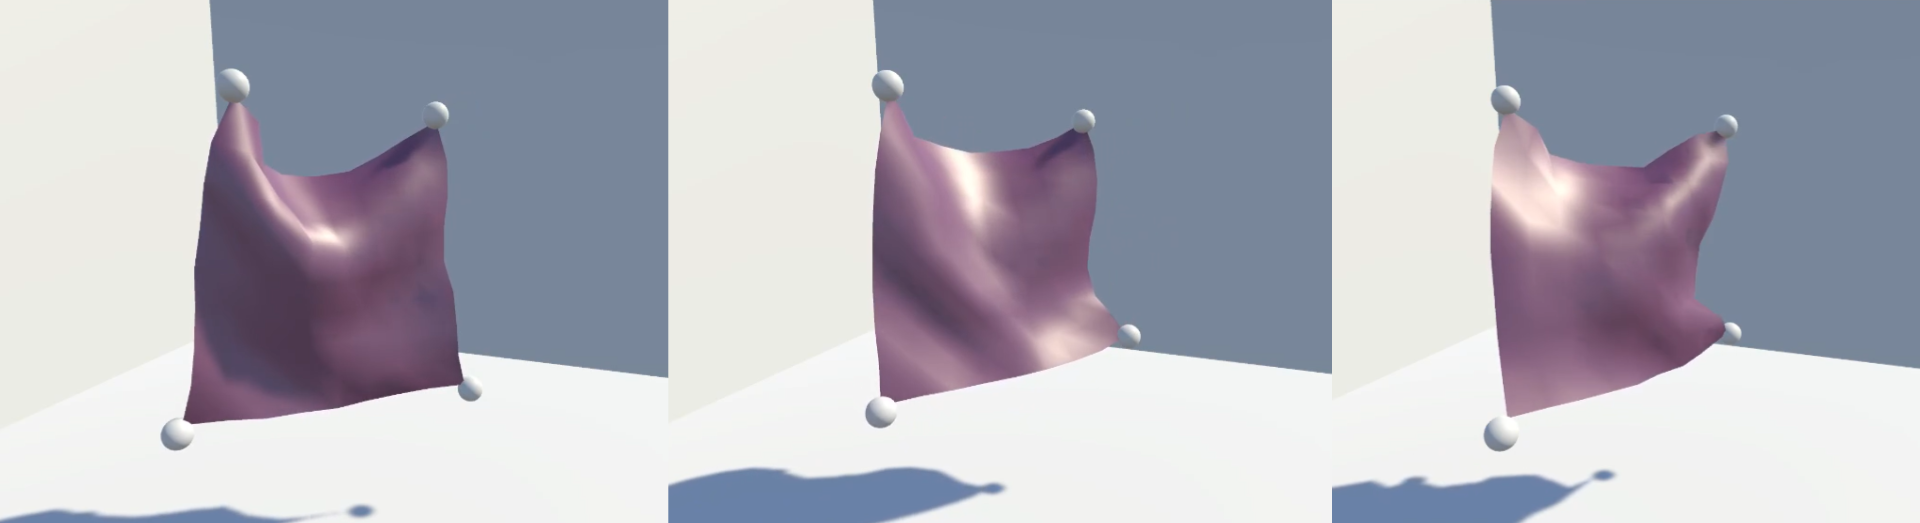
\includegraphics[width=0.8\textwidth]{Imagenes/estatico.png}
	\caption{Ejemplo de la simulación estática implementada.}
	\label{fig:arq}
\end{figure}